\documentclass[12pt,a4paper]{article}
\usepackage[utf8]{inputenc}
\usepackage{amsmath,amssymb}
\usepackage[left=2cm,right=2cm,top=2cm,bottom=2cm]{geometry}
\usepackage{enumitem}
\usepackage{pgfplots}
\pgfplotsset{compat=1.18}

\setlength{\parindent}{0pt}
\setlist[enumerate,1]{leftmargin=*,itemsep=1.2em}
\setlist[enumerate,2]{label=(\alph*),itemsep=0.3em}
\newcommand{\pembahasan}{\par\medskip\textbf{Pembahasan.}\par\smallskip}
\newcommand{\poin}[1]{\hfill\textbf{[#1 poin]}}

\begin{document}

\begin{center}
  \textbf{\Large KALKULUS I (5)}\\[0.2cm]
  \textbf{\large KUIS 1 -- VERSI A}\\[0.3cm]
  \begin{tabular}{|l|l|}
    \hline
    Tanggal     & Selasa, 22 September 2026 \\ \hline
    Durasi      & 100 menit (12.30--14.10)  \\ \hline
    Sifat Ujian & Tutup Buku                \\ \hline
    Dosen       & Helisyah Nur Fadhilah      \\ \hline
  \end{tabular}
\end{center}

\section*{Bagian A. Jawaban Singkat \hfill [20 poin]}
\textit{Setiap soal bernilai 4 poin. Isilah bagian yang kosong dengan jawaban yang tepat.}

\begin{enumerate}
  \item \textbf{Bilangan Real} \poin{4}

    Bilangan $\sqrt{11}$ merupakan bilangan \underline{\hspace{3cm}},
    karena tidak dapat dinyatakan dalam bentuk
    \[
      \frac{a}{b},\qquad a,b\in\mathbb{Z},\quad b\ne 0.
    \]

    \pembahasan
    $11$ bukan kuadrat sempurna. Jadi, $\boxed{\sqrt{11}\text{ adalah bilangan irasional}}$.

  \item \textbf{Nilai Mutlak} \poin{4}

    Tentukan nilai $x$ yang memenuhi persamaan
    \[
      |2x-3|=5
    \]
    dengan menggunakan definisi nilai mutlak.
    Tuliskan jawaban dalam notasi selang.

    \pembahasan
    Gunakan definisi
    \[
      |2x-3|=
      \begin{cases}
        2x-3, & x\ge \frac32,\\
        -(2x-3), & x<\frac32.
      \end{cases}
    \]
    Untuk $x\ge\frac32$, diperoleh $2x-3=5$, sehingga $x=4$.
    Untuk $x<\frac32$, diperoleh $-2x+3=5$, sehingga $x=-1$.
    Keduanya memenuhi syarat masing-masing.
    \[
      \boxed{\mathrm{HP}=\{-1,4\}=[-1,-1]\cup[4,4]}.
    \]
    Selang $[a,a]$ hanya berisi satu titik, yaitu $a$.

  \item \textbf{Persamaan Garis} \poin{4}

    Diberikan persamaan garis
    \[
      3x-2y+6=0.
    \]
    Gradien garis tersebut adalah \underline{\hspace{3cm}}.

    \pembahasan
    Ubah ke bentuk $y=mx+c$:
    \[
      2y=3x+6\quad\Longrightarrow\quad y=\frac32x+3.
    \]
    Jadi, gradiennya $\boxed{m=\frac32}$.

  \item \textbf{Persamaan Lingkaran} \poin{4}

    Diberikan persamaan lingkaran
    \[
      x^2+y^2-8x+6y=11.
    \]
    Tentukan pusat dan jari-jari lingkaran tersebut.

    \pembahasan
    Lengkapi kuadrat:
    \begin{align*}
      (x^2-8x+16)+(y^2+6y+9)&=11+16+9,\\
      (x-4)^2+(y+3)^2&=36.
    \end{align*}
    Jadi, $\boxed{\text{pusat }(4,-3),\quad\text{jari-jari }r=6}$.

  \item \textbf{Operasi pada Fungsi} \poin{4}

    Diberikan $f(x)=2x+1$ dan $g(x)=x^2-3$.
    Tentukan $(f-g)(x)$.

    \pembahasan
    \[
      (f-g)(x)=f(x)-g(x)=(2x+1)-(x^2-3)
      =\boxed{-x^2+2x+4}.
    \]
\end{enumerate}

\newpage
\section*{Bagian B. Esai \hfill [80 poin]}
\textit{Setiap soal bernilai 20 poin. Tunjukkan semua langkah yang diperlukan dalam penyelesaian.}

\begin{enumerate}
  \item \textbf{Pertidaksamaan Nilai Mutlak} \poin{20}

    Selesaikan pertidaksamaan
    \[
      \left|\frac{2x+1}{3}\right|>\frac43.
    \]
    Tentukan himpunan penyelesaiannya dan tuliskan dalam notasi selang.

    \pembahasan
    Karena penyebutnya positif, kita dapat menulis
    $\left|\frac{2x+1}{3}\right|=\frac{|2x+1|}{3}$.
    Kalikan kedua ruas dengan $3$. Tanda pertidaksamaan tetap karena $3>0$.
    \[
      \frac{|2x+1|}{3}>\frac43\iff |2x+1|>4.
    \]
    Nilai mutlak menyatakan jarak suatu bilangan dari nol.
    Agar jaraknya lebih dari $4$, bilangan itu harus kurang dari $-4$ atau lebih dari $4$.
    Jadi, ada dua kemungkinan:
    \begin{align*}
      2x+1<-4 &\iff 2x<-5\iff x<-\frac52,\\
      2x+1>4 &\iff 2x>3\iff x>\frac32.
    \end{align*}
    Kedua hasil digabung dengan kata ``atau'', karena cukup salah satu kondisi yang terpenuhi.
    Maka himpunan penyelesaiannya adalah
    \[
      \boxed{\mathrm{HP}=\left\{x\in\mathbb{R}\mid x<-\frac52
        \text{ atau }x>\frac32\right\}}.
    \]
    Dalam notasi selang,
    \[
      \boxed{\mathrm{HP}=\left(-\infty,-\frac52\right)
        \cup\left(\frac32,\infty\right)}.
    \]
    Titik $-\frac52$ dan $\frac32$ tidak termasuk.
    Pada kedua titik itu, nilai mutlaknya tepat $4$, sedangkan soal meminta nilai yang lebih besar dari $4$.

  \newpage
  \item \textbf{Persamaan Garis dengan Parameter $k$} \poin{20}

    Diberikan dua garis dan titik $P(-2,3)$:
    \[
      L_1:(k+2)x-y-3=0,\qquad
      L_2:3x+(k-2)y+6=0.
    \]
    Tentukan:
    \begin{enumerate}
      \item nilai $k$ jika garis $L_2$ tegak lurus terhadap $L_1$;
      \item persamaan garis $L$ yang melalui titik $P$ dan sejajar dengan $L_1$;
      \item persamaan garis yang melalui titik $P$ dan tegak lurus terhadap $L_1$.
    \end{enumerate}

    \pembahasan
    \begin{enumerate}
      \item Untuk mencari gradien, ubah persamaan garis ke bentuk $y=mx+c$.
        Koefisien $x$ pada bentuk ini adalah gradiennya.
        \begin{align*}
          L_1:\quad y&=(k+2)x-3,\\
          L_2:\quad y&=-\frac{3}{k-2}x-\frac{6}{k-2}\qquad(k\ne2).
        \end{align*}
        Jadi, gradien kedua garis adalah
        \[
          m_1=k+2,\qquad m_2=-\frac{3}{k-2}\quad(k\ne2).
        \]
        Dua garis dengan gradien terdefinisi saling tegak lurus jika $m_1m_2=-1$.
        Substitusikan kedua gradien:
        \begin{align*}
          -\frac{3(k+2)}{k-2}=-1
          &\iff 3(k+2)=k-2\\
          &\iff 3k+6=k-2\iff 2k=-8.
        \end{align*}
        Maka $\boxed{k=-4}$.
        Untuk nilai ini, $m_1=-2$ dan $m_2=\frac12$.
        Hasil kalinya $-1$, sehingga syarat tegak lurus terpenuhi.

        Nilai $k=2$ perlu diperiksa terpisah karena membuat penyebut gradien nol.
        Saat $k=2$, garis $L_2$ menjadi $x=-2$, yaitu garis vertikal.
        Garis yang tegak lurus dengannya harus horizontal.
        Namun, $L_1$ bergradien $4$, sehingga $k=2$ bukan solusi.

      \item Gunakan $k=-4$ dari bagian (a), sehingga $m_1=-2$.
        Garis sejajar memiliki gradien yang sama, jadi gradien $L$ juga $-2$.
        Gunakan bentuk titik--gradien $y-y_0=m(x-x_0)$ dengan $P(-2,3)$:
        \begin{align*}
          y-3&=-2\bigl(x-(-2)\bigr)=-2(x+2),\\
          y&=-2x-1.
        \end{align*}
        Jadi, persamaan garisnya $\boxed{2x+y+1=0}$.

      \item Garis yang dicari tegak lurus terhadap $L_1$, sehingga $(-2)m=-1$.
        Jadi, gradiennya $m=\frac12$.
        Gunakan kembali titik $P(-2,3)$:
        \begin{align*}
          y-3&=\frac12(x+2),\\
          2y-6&=x+2.
        \end{align*}
        Setelah semua suku dipindahkan ke satu ruas, diperoleh
        $\boxed{x-2y+8=0}$.
    \end{enumerate}

  \newpage
  \item \textbf{Grafik Fungsi dan Pergeseran} \poin{20}

    Diberikan fungsi dasar $f(x)=x^2$.
    Gambarkan grafik $g(x)=(x-2)^2-3$ dengan menggunakan grafik $f(x)=x^2$ sebagai acuan.
    Kemudian:
    \begin{enumerate}
      \item gambarkan grafik $g(x)$;
      \item tentukan arah dan besar pergeseran;
      \item tentukan titik puncak grafik $g(x)$;
      \item tentukan domain $g(x)$;
      \item tentukan range $g(x)$.
    \end{enumerate}

    \begingroup
    \setlength{\abovedisplayskip}{6pt}
    \setlength{\belowdisplayskip}{6pt}
    \setlength{\abovedisplayshortskip}{4pt}
    \setlength{\belowdisplayshortskip}{4pt}
    \pembahasan
    \begin{enumerate}
      \item Grafik dasar $f(x)=x^2$ adalah parabola yang terbuka ke atas.
        Puncaknya berada di $(0,0)$.
        Pada $g(x)=(x-2)^2-3$, koefisien suku kuadrat tetap $1$.
        Jadi, bentuk dan arah buka parabolanya tetap sama.

        Untuk membantu menggambar, substitusikan beberapa nilai $x$:
        \[
          \begin{array}{c|rrrrr}
            x & 0 & 1 & 2 & 3 & 4\\ \hline
            g(x) & 1 & -2 & -3 & -2 & 1
          \end{array}
        \]
        Titik-titik tersebut simetris terhadap garis $x=2$.
        Hubungkan dengan kurva parabola yang halus seperti pada gambar.

        \begin{center}
          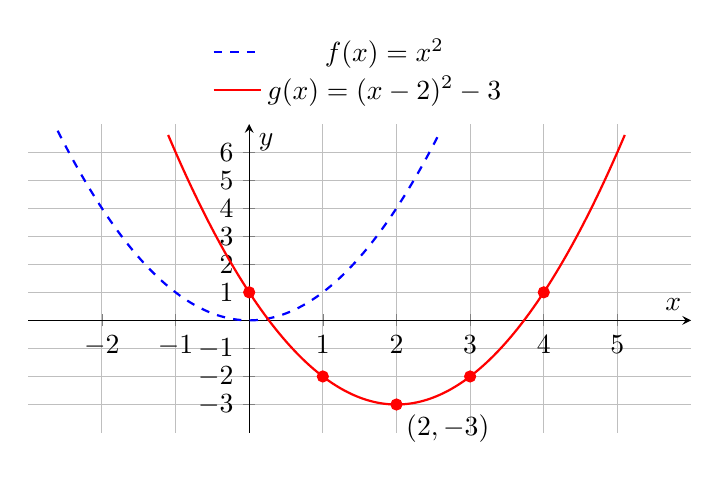
\begin{tikzpicture}
            \begin{axis}[
              width=10cm,height=5.5cm,
              axis lines=middle,
              xlabel={$x$},ylabel={$y$},
              xmin=-3,xmax=6,ymin=-4,ymax=7,
              xtick={-2,-1,0,1,2,3,4,5},
              ytick={-3,-2,-1,0,1,2,3,4,5,6},
              grid=major,samples=120,
              legend style={at={(0.5,1.03)},anchor=south,draw=none},
              clip=false
            ]
              \addplot[blue,dashed,thick,domain=-2.6:2.6] {x^2};
              \addlegendentry{$f(x)=x^2$}
              \addplot[red,thick,domain=-1.1:5.1] {(x-2)^2-3};
              \addlegendentry{$g(x)=(x-2)^2-3$}
              \addplot[red,only marks,mark=*]
                coordinates {(0,1) (1,-2) (2,-3) (3,-2) (4,1)};
              \node[below right] at (axis cs:2,-3) {$(2,-3)$};
            \end{axis}
          \end{tikzpicture}
        \end{center}

      \item Penggantian $x$ menjadi $x-2$ menggeser grafik $2$ satuan ke kanan.
        Pengurangan $3$ di luar kuadrat menurunkan semua nilai fungsi sebesar $3$.
        Jadi, grafik $f$ digeser
        $\boxed{2\text{ satuan ke kanan dan }3\text{ satuan ke bawah}}$.
        Setiap titik $(a,a^2)$ pada $f$ berpindah ke $(a+2,a^2-3)$ pada $g$.

      \item Bentuk puncak parabola adalah $y=(x-h)^2+k$, dengan puncak $(h,k)$.
        Pada soal, $h=2$ dan $k=-3$.
        Maka titik puncaknya $\boxed{(2,-3)}$.
        Ini juga hasil pergeseran puncak awal $(0,0)$.

      \item Domain adalah himpunan nilai $x$ yang dapat dimasukkan ke fungsi.
        Operasi pengurangan dan pengkuadratan terdefinisi untuk setiap bilangan real.
        Karena itu, tidak ada pembatasan nilai $x$.
        Jadi, $\boxed{D_g=\mathbb{R}=(-\infty,\infty)}$.

      \item Kuadrat suatu bilangan real selalu tak negatif, sehingga $(x-2)^2\ge0$.
        Akibatnya, $g(x)=(x-2)^2-3\ge-3$.
        Nilai minimum $-3$ tercapai saat $x=2$.
        Parabola terbuka ke atas, sehingga semua nilai di atas $-3$ juga tercapai.
        Jadi, range atau daerah hasilnya adalah $\boxed{R_g=[-3,\infty)}$.
        Tanda kurung siku dipakai karena nilai $-3$ termasuk daerah hasil.
    \end{enumerate}
    \endgroup

  \newpage
  \item \textbf{Komposisi Fungsi} \poin{20}

    Diberikan
    \[
      g(x)=\sqrt{x+1}
      \qquad\text{dan}\qquad
      (f\circ g)(x)=\sqrt{3x-2}.
    \]
    Tentukan:
    \begin{enumerate}
      \item $f(\sqrt{3})$;
      \item domain dari $f(x)$;
      \item $(g\circ f)(x)$;
      \item domain dari $(g\circ f)(x)$.
    \end{enumerate}
    \textit{Petunjuk: $D_{g\circ f}=\{x\in D_f\mid f(x)\in D_g\}$.}

    \pembahasan
    Komposisi $(f\circ g)(x)$ berarti $f(g(x))$.
    Karena $g(x)=\sqrt{x+1}$, informasi pada soal dapat ditulis sebagai
    \[
      f\bigl(\sqrt{x+1}\bigr)=\sqrt{3x-2}.
    \]
    Untuk mencari rumus $f$, misalkan masukannya $t=\sqrt{x+1}$.
    Kuadratkan kedua ruas, sehingga $t^2=x+1$ atau $x=t^2-1$.
    Substitusikan ke ruas kanan:
    \begin{align*}
      f(t)&=\sqrt{3(t^2-1)-2}\\
          &=\sqrt{3t^2-3-2}=\sqrt{3t^2-5}.
    \end{align*}
    Untuk jawaban berikut, gunakan $f(x)=\sqrt{3x^2-5}$ dengan domain alaminya.
    \begin{enumerate}
      \item Masukkan $\sqrt3$ sebagai nilai argumen fungsi $f$:
        \[
          f(\sqrt3)=\sqrt{3(\sqrt3)^2-5}
            =\sqrt{3\cdot3-5}=\sqrt4=\boxed{2}.
        \]
        Nilai di dalam akar adalah $4\ge0$, sehingga hasil ini terdefinisi.

      \item Agar $f(x)$ bernilai real, bilangan di dalam akar harus tak negatif:
        \[
          3x^2-5\ge0\iff x^2\ge\frac53
          \iff |x|\ge\sqrt{\frac53}.
        \]
        Artinya, $x\le-\sqrt{\frac53}$ atau $x\ge\sqrt{\frac53}$.
        Kedua batas diperbolehkan karena menghasilkan akar nol.
        Jadi,
        \[
          \boxed{D_f=\left(-\infty,-\sqrt{\frac53}\right]
            \cup\left[\sqrt{\frac53},\infty\right)}.
        \]

      \newpage
      \item Pada $(g\circ f)(x)$, fungsi $f$ dikerjakan lebih dahulu.
        Hasilnya menjadi masukan fungsi $g$.
        Karena $g(u)=\sqrt{u+1}$, kita peroleh
        \[
          (g\circ f)(x)=g(f(x))=\sqrt{f(x)+1}
          =\boxed{\sqrt{\sqrt{3x^2-5}+1}}.
        \]

      \item Domain komposisi harus memenuhi dua syarat.
        Pertama, $x\in D_f$ agar fungsi dalam dapat dihitung.
        Kedua, $f(x)\in D_g$ agar hasilnya dapat dimasukkan ke fungsi luar.

        Untuk $g(u)=\sqrt{u+1}$, syaratnya $u\ge-1$.
        Jadi, $D_g=[-1,\infty)$.
        Sementara itu, $f(x)=\sqrt{3x^2-5}\ge0$ untuk setiap $x\in D_f$.
        Maka $f(x)$ selalu berada di $D_g$.
        Tidak ada pembatasan tambahan dari fungsi luar, sehingga
        \[
          \boxed{D_{g\circ f}=D_f
            =\left(-\infty,-\sqrt{\frac53}\right]
            \cup\left[\sqrt{\frac53},\infty\right)}.
        \]
    \end{enumerate}
    \textit{Catatan: akar pada $(f\circ g)(x)$ mensyaratkan $x\ge\frac23$.
    Karena $t=\sqrt{x+1}$, masukan $f$ yang diketahui dari soal hanya
    $t\ge\sqrt{5/3}$. Jawaban domain di atas memakai perluasan rumus
    $f(t)=\sqrt{3t^2-5}$ ke domain alaminya.}
\end{enumerate}

\end{document}
